\documentclass{l4proj}

% put any additional packages here

\definecolor{dkgreen}{rgb}{0,0.6,0}
\definecolor{gray}{rgb}{0.5,0.5,0.5}
\definecolor{mauve}{rgb}{0.58,0,0.82}

\lstset{frame=tb,
  language=Scala,
  aboveskip=3mm,
  belowskip=3mm,
  showstringspaces=false,
  columns=flexible,
  basicstyle={\small\ttfamily},
  numbers=left,
  numberstyle=\tiny\color{gray},
  keywordstyle=\color{blue},
  commentstyle=\color{dkgreen},
  stringstyle=\color{mauve},
  breaklines=true,
  breakatwhitespace=true,
  tabsize=2
}
%

\begin{document}


%==============================================================================
%% METADATA
\title{Level 4 Project Report}
\author{Euan McGrevey}
\date{March 20, 2020}

\maketitle

%==============================================================================
%% ABSTRACT
\begin{abstract}

    Two keys challenges have arisen since the advent of highly parallel computer architectures: Programmability and Performance Portability. This project used Lift by \citet{steuwer_improving_nodate} as a template to explore how these issues could be addressed. Specifically it explores the Lift rewrite rule model for optimising programs applied to encode mathematical relations on expressions, and how efficiently rewriting of these could be done. The developed interface for rewriting has proven to useful.

\end{abstract}

%==============================================================================

% EDUCATION REUSE CONSENT FORM
% If you consent to your project being shown to future students for educational purposes
% then insert your name and the date below to  sign the education use form that appears in the front of the document. 
% You must explicitly give consent if you wish to do so.
% If you sign, your project may be included in the Hall of Fame if it scores particularly highly.
%
% Please note that you are under no obligation to sign 
% this declaration, but doing so would help future students.
%
\def\consentname {Euan McGrevey} % your full name
\def\consentdate {30 January 2020} % the date you agree
%
\educationalconsent


%==============================================================================
\tableofcontents

%==============================================================================
%% Notes on formatting
%==============================================================================
% The first page, abstract and table of contents are numbered using Roman numerals and are not
% included in the page count. 
%
% From now on pages are numbered
% using Arabic numerals. Therefore, immediately after the first call to \chapter we need the call
% \pagenumbering{arabic} and this should be called once only in the document. 
%
% Do not alter the bibliography style.
%
% The first Chapter should then be on page 1. You are allowed 40 pages for a 40 credit project and 30 pages for a 
% 20 credit report. This includes everything numbered in Arabic numerals (excluding front matter) up
% to but excluding the appendices and bibliography.
%
% You must not alter text size (it is currently 10pt) or alter margins or spacing.
%
%
%==================================================================================================================================
%
% IMPORTANT
% The chapter headings here are **suggestions**. You don't have to follow this model if
% it doesn't fit your project. Every project should have an introduction and conclusion,
% however. 
%
%==================================================================================================================================
\chapter{Introduction} \label{introduction}

% reset page numbering. Don't remove this!
\pagenumbering{arabic} 


Lift is a research project that strives to ease the problems of Performance Portability (Having fast code on different computer architectures) and Programmability (How hard it is to write the code).

Performance Portability is a challenge for programmers. It is inescapable due to the nature of hardware vendors designing their processors differently from one another. Extensive performance guides are published by each, detailing the best ways to write code which takes advantage of their processors. Ultimately this leads to programmers writing low level code that works really well on one specific architecture, and works worse or may not even compile on other architectures.

Programmability is another such issue that comes with writing optimised code. In current industry standard parallel programming models such as OpenCL, optimisations are typically ad hoc and result in unintuitive, hard to read code. Not only does this put a significant burden on the programmer, but it results in the code being inherently unmaintainable.


Compilers present the opportunity to solve or relieve both of these issues.
%This increases the burden on the programmer to write fast code as when run on different machines, it may run slower or even not at all.

This project started out by aiming to investigate how the application of Lift's rewrite rules could improve the performance of common image processing techniques, such as blurring and up-scaling. However, over the course of the first semester of project work, it became apparent that this was much harder than first anticipated, and so the scope of the project was changed to "Examining the transformation of Lift expressions which model Arithmetic using rewrite rules". 

The transformation of expressions using rewrite rules in Lift is of particular interest for Performance Portability and Programmability as the rules encode optimisation and implementation choices. The high level Lift code that the programmer writes does not in any way express to the compiler how the code will be executed, just the abstract solution. 


For example, the absolute summation of values in an array can be written in high level Lift as:
\begin{lstlisting}[caption={High level Description of Absolute Summation \citep{steuwer_generating_icfp}}, label={lst:Lift high level asum}]
    asum = reduce (+) 0  map abs 
\end{lstlisting}
    
Note the map and reduce functional primitives that are exposed to the programmer. This allows for a concise and readable definition of a function, that does not describe how it is actually applied. After running the high level code through Lift's compiler, we can get several low level implementations for different hardware architectures, such as Listing \ref{lst:Low level asum}, which is targeted for an Nvidia GPU.


\begin{lstlisting}[mathescape, caption={Low Level implementation of Listing \ref{lst:Lift high level asum}  \citep{steuwer_generating_icfp}, targeting an Nvidia GPU}, label={lst:Low level asum}]
$ \lambda $x.(reduceSeq  join  join  mapWorkgroup (
    toGlobal mapLocal (reduceSeq ((a, b). a + (abs b)) 0) reorderStride 2048
)  split 128  split 2048) x
\end{lstlisting}
    
Note the 'reduce' and 'abs' functions are still present, but the majority of the function is spent encoding optimisations with hard-coded numbers to denote how to lay out data in memory and how to split work between compute units on the GPU. As these numbers are specific to a particular Nvidia GPU, the optimisations do not carry over to other architectures, making it inherently unportable. 


Still, why might it be useful to decouple what code does from how it does it? Suppose we have a high level algorithm as in Listing \ref{lst:Lift high level asum}. We could also write a low level optimized implementation separately. As the latter will tend to implement hardware specific and ad hoc techniques to gain maximal performance, there is often a lot of 'noise' and obfuscation in the code that can make it difficult to see that it still is in fact a valid implementation of the original high level algorithm, as with Listing \ref{lst:Low level asum}. 

Here is where Lift uses rewrite rules, which encode these specific implementation optimisations, to tackle Programmability. The programmer need only specify a high level algorithm such as Listing \ref{lst:Lift high level asum}, and decide which target architecture they would like, and the optimised implementation code is generated. 
As a bonus, this process can be done multiple times to generate many low level implementations that are optimised for different architectures, aiding the Performance Portability challenge.


%This is where rewrite rules, and this project, come in. Through the use of Lift's rewrite rules, we can in theory transform the easily programmable high level absolute summation program into the low level optimised version, with the guarantee that semantically the two programs are the same. In this way, we can also be confident there is no undefined behaviour or side effects when running the optimised version, thus tackling the programmability challenge, as we need not ever write hardware specific code. 
%If the process of generating low level programs from high level specifications can be automated, then Performance Portability YYY, as we can generate as many implementations as needed for whatever desired hardware, needing only to specify the rules used in the transformation.

% Maybe a small para about this project looking at rewrite rules to prove equivalence between high level and low level implementations by examining a constrained problem.

In this project, we develop tooling to help explore the application of Lift-style rewrite rules.

%==================================================================================================================================
\chapter{Background} \label{background}

In this section we take a look at Halide, an image processing language that tries to tackle performance portability and programmability in an alternative way to Lift. We then compare this model to Lift, a more general language that aims to optimise programs completely transparently from the user.


\section{Halide}

Halide is a language embedded in C++ designed to target image processing pipelines. As image processing techniques often require applying the same function to many different pixels of an image, exploiting data parallelism is a natural way to enhance performance.

Halide attempts to tackle Performance Portability by decoupling 'what' the program does from 'how' it does it. In a Halide program, what the program does is called the 'Algorithm', and how it does it is called the 'Schedule'

The Schedule, written by the programmer, explains to the compiler how to allocate memory and how to order the instructions to achieve whatever is optimal for the programmer, be it memory usage or runtime.

\begin{lstlisting}[caption={A Halide program for blurring an image\citep{Halide_Website}}, language={C++}]
Func blur_3x3(Func input) {
  Func blur_x, blur_y;
  Var x, y, xi, yi;

  // The algorithm - no storage or order
  blur_x(x, y) = (input(x-1, y) + input(x, y) + input(x+1, y))/3;
  blur_y(x, y) = (blur_x(x, y-1) + blur_x(x, y) + blur_x(x, y+1))/3;

  // The schedule - defines order, locality; implies storage
  blur_y.tile(x, y, xi, yi, 256, 32)
        .vectorize(xi, 8).parallel(y);
  blur_x.compute_at(blur_y, x).vectorize(x, 8);

  return blur_y;
}
\end{lstlisting}

We can see how the above example illustrates Halide's approach to solving the programmability problem of parallel systems. The actual algorithm itself is entirely decoupled from any notion of optimisation, requiring the programmer only to state what has to be done.

This enables the programmer to write different schedules which optimise a given program for different hardware architectures of their choosing, with each schedule taking advantage of the chosen architecture's design. This makes Halide a suitable choice when there are only a handful of target architectures for a product.


However, there are some major drawbacks. Primarily, Halide is only intended to be used for image processing pipelines. This intentional limit on the problem space is what allows it to be a practical platform to program with. Its ambition is curbed so that it can still be a relatively small and practical language for developers who need it.

Secondly, it does require the programmer to write the schedule, which is often far more difficult than writing the actual program. And if you want your program to be used on many different architectures, then you have to write a separate schedule for each. This makes it unsuitable for use in mainstream end-user products, since they will inevitably use myriad different types of computers.


Lift aims to go for even more ambitious heights, and addresses both of these issues.
       
\section{Lift}

Lift aims to be a more ambitious research project. The language constructs (such as ???) allows more than just image processing applications to be written. Compared with Halide, Lift has a high level DSL built in Scala (cite??) which is used by programmers to write code. However, the optimisation process is completely transparent in Lift.

The Lift high level language exposes to the programmer common functional primitives with which to write programs.

\begin{lstlisting}[caption={An example of Matrix Multiplication written in SkelCL\citep{steuwer_improving_nodate}, the predecessor to Lift}, keywords={const, Vector, float, int, Matrix, return}]

Matrix<float> mm(const Matrix<float>& A, const Matrix<float>& B) {
    skelcl::init();
    auto mm = allpairs(
    [](const Vector<float>& a, const Vector<float>& b) {
        float c = 0.0f;
        for (int i = 0; i < a.size(); ++i)
            c += a[i] * b[i];
        return c; });
    return mm(A, B); }

\end{lstlisting}

[TODO: Talk about the listing here, highlight the allpairs function as one of the high level patterns that allows a myriad of optimisation choices behind the scenes]

How then are we able to optimise code? In Lift, this is done automatically through what are called rewrite rules. The Lift compiler takes program source code written by a developer and automatically generates several low level implementations, for example it could generate both C code and OpenCL code that do the same thing. The compiler may also produce different implementations of the code in the same language, such as OpenCL, where there might be implementations which are optimised for running on an AMD GPU or a multi-core Intel CPU.

How does this work? = Rewrite rules encode optimisations


\begin{lstlisting}[caption={The RewriteResult trait definition taken directly from Lift (omitted are functions for retrieving value from the wrapper object, not used in this project)}]
sealed trait RewriteResult[P] {
  ...
}

case class Success[P](p: P) extends RewriteResult[P] {
  ...
}

case class Failure[P](s: Strategy[P]) extends RewriteResult[P] {
  ...
}
\end{lstlisting}




In this way, Lift offers a flexible solution to the programmability problem, completely eliminating the programmer from the optimisation process, and therefore removing the burden of optimising and maintaining low level code. 

\section{Guidance}
\begin{itemize}    
    \item
      Don't give a laundry list of references.
    \item
      Tie everything you say to your problem.
    \item
      Present an argument.
    \item Think critically; weigh up the contribution of the background and put it in context.    
    \item
      \textbf{Don't write a tutorial}; provide background and cite
      references for further information.
\end{itemize}







%==================================================================================================================================
\chapter{Requirements} \label{requirements}

\section{Requirements from motivation}
Going back to our basic question, "How can we find out if we can transform one expression into another?", we will establish what exactly is required in order to answer this question, as well as the constrained version of this question that this project aims to answer.
 
Based on this question, we might want to establish a framework or suite of functions that manage transformations automatically, to save much time and effort.
 
For such an interface, we can draw up the following requirements. We want to know:
\begin{itemize}
    \item Which rules are used in the transformation of expressions.
    \item What order they are applied in.
    \item Where in the program AST they are applied.
    \item That certain rule applications don't change the meaning of the program (semantic preservation).
    \item It can be arbitrarily precise (that is, if you can get to the goal, the interface should be able to tell you definitively, with no false negatives).
    \item It is efficient.
\end{itemize}
 
This is a lot for a single project, so we will constrain our requirements to make it more manageable.
Specifically, we will throw away efficiency for the sake of ease of programming. 
And we will not be rigorous when it comes to proving the application of certain rewrite rules do not alter the meaning of the program. Such proofs may be suitable for further work.
%For ensuring that a rule application will not change the semantic meaning of the expression is more difficult, and doing it 100\% is beyond the scope of this project. It is not true in general that rule application will not change the semantic meaning of the expression it operates on. However, for this project, we can restrict ourselves to only using rewrite rules that encode equivalences, such as in Section \ref{evaluation}. As well as only given these rules well formed and meaningful expressions to operate on. There is no type checking or semantic analysis provided for the purposes of this project; It is assumed.

 
 
\section{Success Criteria}
In order to know when we have met achieved our constrained requirements, let us specify some more concrete goals:
\begin{itemize}
    \item We would like to develop a series of functions which transform expressions
    \item For our functions we would like them to tell us precisely which rules are used in the transformation, as well as the order of the rule applications.
    \item Furthermore, the functions should output the location where the rule applications happen, in such a way that the transformations can be replicated exactly.
    \item Finally, our functions must be able to take arbitrary start and goal expressions, and any number of rewrite rules to work with.
\end{itemize}
 
 
If we can achieve this, then we will have a primitive version of the universal expression transformer that satisfies requirements 1,2, and 3. To satisfy requirement 5, we can allow our functions a stop parameter which will only permit the function to allow so many rule applications before giving up (that is, if a transformation can't be done in X rule applications or less, it will be treated as though it is impossible).
 
 
In section 4, we design a series of functions that handle the traversal of a more abstract data type, the tree. 

These functions are then implemented in section 5.

Section 6 uses our traversal functions with a set of rewrite rules for Arithmetic for a case study evaluating how well we have fulfilled our success criteria.
 
%==================================================================================================================================
\chapter{Design} \label{design}

As Lift is a DSL built in Scala, we use Scala in this project for ease of extensibility.

\section{Data Representation}

\subsection{Abstract Syntax Trees}

One of the steps early on during the compilation of a program is the reduction of the source code to an Abstract Syntax Tree (AST). An AST is a representation of a program's source code with all unnecessary information expunged. Thus this project uses Trees as a basis to represent expressions since they can model the design of ASTs and may be extended in future work to accommodate more program-like features, eventually modeling entire programs, in order to answer our question presented in Section \ref{introduction}. How can we be sure that a low level optimised implementation of a high level algorithm is correct?


\subsection{Expressions}

Our trees are modeled as a trait, with two possible values, either an empty node, or a node with a value and two children, which may be empty nodes themselves.

\begin{minipage}{\linewidth}
\begin{lstlisting}[caption={Definition of a Tree}]
sealed trait Tree {}

case class Node(var left: Tree, var value: String, var right: Tree) extends Tree {}

case object EmptyNode extends Tree {}
\end{lstlisting}
\end{minipage}

For the purposes of making implementation easier, our trees are strictly binary. Each node has a String value. This string can be anything, and is used to encode information about the node, and can be used to pattern match in rewrite rules or elsewhere.
These trees that we use do not need to encode a full program AST. For the purposes of this project, we can use them to represent a smaller set of arbitrary ASTs of computations.


Since our goal is to have a universal expression transformer, we need some way of traversing a given tree as well as a way of deciding when a rule has been successfully applied to a node in the tree.







\section{Rewrite Rules}

% TODO: Is this answered?
%Section 4. What is applyEverywhere supposed to be doing. What does it mean. Rather than how it does it.
%Could have a small diagram of tree illustrating this

Also referred to as a Strategy (this is what they are called in Lift), a rewrite rule somehow transforms an expression whilst maintaining its meaningfulness.

Specifically, rewrite rules are functions, parameterised over some type P, which take an object of type P as input and return a RewriteResult, which is also parameterised over P.

This make sense, the rewrite rule interface is type-agnostic, and each individual rule only works on whatever data type it wants. This allows a small and simple interface. Listing \ref{lst:Strategy} lays out this definition.

\begin{lstlisting}[caption={Definition of a Rewrite Rule as a type alias}, label={lst:Strategy}]
type Strategy[P] = P => RewriteResult[P]
\end{lstlisting}


\subsection{Rewrite Result}

Listing \ref{lst:RewriteResult} provides the interface for rewrite rules, RewriteResult, which allows us the ability to decide whether rule applications are successes or failures.

We use a Scala trait to represent the result of applying rewrite rules to a node, with case classes for Success and Failure. This trait is primarily just a wrapper for the result value used for pattern matching purposes, as we can decide what to do when applying a rule to a node does not work via pattern matching over these two case classes.

\begin{lstlisting}[caption={Definition of RewriteResult trait for handling the result of applying rewrite rules}, label={lst:RewriteResult}]
// omitted are functions for retrieving the result of the rule application 
sealed trait RewriteResult[P] {...}

case class Success[P](p: P) extends RewriteResult[P] {...}

case class Failure[P](p: P) extends RewriteResult[P] {...}
\end{lstlisting}





\subsection{Rule Application}

Using these means, [how do we achieve our goals as set in section 3]





Listing \ref{lst:Rewrite Rule Example} provides an example rewrite rule, which takes an empty node and turns it into a tree with a left child.

\begin{lstlisting}[caption={A Rewrite rule which takes an Empty node, and replaces it with a Node with one left child}, label={lst:Rewrite Rule Example}]
case class Section4Example() extends Strategy[Tree] = {
    def apply(e: Tree): RewriteResult[Tree] = e match {
        case EmptyNode => Success(Node(Node(EmptyNode, "x", EmptyNode), "y", EmptyNode))
        case _ => Failure(Section4Example())
    }
}
\end{lstlisting}

Note the return values are wrapped in either Success() or Failure() to indicate whether the rule application worked.



To help visualise the effect of applying rewrite rules, the application of the rule presented in Listing \ref{lst:Rewrite Rule Example} can be visualised as in Figure \ref{fig:RewriteRule_Application_Example}

\begin{figure}
    \centering
    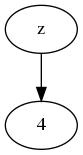
\includegraphics[scale=0.5]{images/Section4Example0}
    \hspace{2cm}
    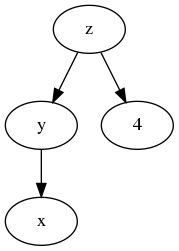
\includegraphics[scale=0.5]{images/Section4Example1}
    \caption{Before and after application of the rule in Listing \ref{lst:Rewrite Rule Example} to the empty left child of the left expression}
    \label{fig:RewriteRule_Application_Example}
\end{figure}














Now that we have talked about our tree representation and how rewrite rules work, we can discuss the traversal functions that will make up our interface for exploring the application of rewrite rules.

\section{Traversals}

As our trees are binary, and because trees themselves are naturally recursive, our traversal functions become much more straightforward, since we only need to decide what happens to a single node and both its children. % take out? Seems out of place. Maybe refactor

We now go through each of our success criteria as in chapter \ref{requirements}, and design a way in which we can meet them.


Firstly, using the definition of our rewrite rules, they are functions which return a rewrite result. Thus we can answer whether a rule application was successful by pattern matching on the return value, which will either be a Success or a Failure. Therefore, we can design a simple function which takes a start and goal expression and one rewrite rule, and traverses the start expression, trying to apply the rule to each node, and on a Success, we can check whether the result is the goal. If it is then we know the transformation is possible. If not, then we can simply continue the traversal until we run out of nodes, in which case it is also not possible.


% this is our applyOnce function. Refactor \ref{todothis} to refer to this earlier definition rather than restate
This is the simplest version of our goal, as it only takes one rewrite rule, does not tell you where the rule application happened if successful, and only has an exploration depth of one. That is, if you could get to the goal expression but it took two rule applications, then the function would still return false.


For keeping track of which rules are used in the process of transforming one expression into another, as well as the order in which they are applied, we can maintain an ordered sequence of rules to represent the order of rule application.


Returning the location of where in an expression a rule is applied is a little tougher, since in our design we do not have a unique identifier associated with each node in an expression. Thus, we must develop another way. Our solution is to design two functions. 
\begin{itemize}
\label{todothis}
    \item applyOnce, which traverses an expression, trying to apply a given rule to each node, stopping on the first successful application, or failing after all nodes fail. 
    \label{TODO} % Use a diagram here to show example traversals for both these functions on the same expression.
    \item And applyOnceWithSkip, which does the same as applyOnce, but is provided with a number denoting how many successful rule applications to skip over during its traversal.
\end{itemize}

If we choose to do a preorder traversal for both of these functions, then the order of rule application attempts will always be the same. Thus, when there are many potential nodes to which a given rule can be applied, this 'skip' number will allow us to recreate the same transformation, by doing a preorder traversal over the expression and skipping that many successful applications, after which point we will be at the desired location in the expression.


Finally, we do not need to do any work to allow our functions to take arbitrary start and goal expressions, and in order for them to take any number of rewrite rules, we can include a Set of rewrite rules as a parameter.


%==================================================================================================================================
\chapter{Implementation} \label{implementation}


PLAN:::
Need explanation at the higher level. What is the effect of these rules if I apply them (VISUALISATION).



Each node in our tree can be an operation or an operand, and the precedence of operators corresponds to depth in the tree. Each operation node has two children, which are its operands, and each child may be another operation node. 

Note that we do not place any restriction on what an operand may be, which allows the flexibility of representing Algebraic terms, where operands may be letters such as "A" or "B". This comes at the cost of not checking correctness of expressions, to ensure they are well formatted or meaningful. For example, you could have a node with value "4" that has two children "3" and "5". This may not make any sense, but it is not checked for.






\section{Traversal Function Implementations}

Here is a presentation of the functions implementations for the functions laid out in Section \ref{design}. Each one builds on the previous until we reach our goal of having an arbitrarily precise function that outputs whether it is possible to go from one expression to another, and provides a means to replicate the steps it found to do so.


\subsection{applyOnce and applyOnceWithSkip}

We implement two of the functions from our design that will enable us to replicate the application of a rewrite rule at a particular position in an expression.

applyOnce, referred to in Section \ref{design}, is the most constrained version of the problem scope, where we want to answer whether we can apply \emph{one} rule, \emph{exactly once}.  

Listing \ref{lst:applyOnce} provides the implementation for this function.

\begin{lstlisting}[caption={Function which applies a given rule to only one point in a given tree, returning the transformed tree on a Success or the original on a Failure}, label={lst:applyOnce}]
    def applyOnce(t: Tree, r: Strategy[Tree]): RewriteResult[Tree] = {
      r(t) match { // try the current node
        case Success(newT) => Success(newT)
        case Failure(_) =>
          t match {
            case EmptyNode => Failure(r) // Failure returns
            case Node(ln, s, rn) =>
              // consider left child...
              applyOnce(ln, r) match {
                case Success(newlT) => Success(Node(newlT, s, rn))
                // otherwise, try the right subtree
                case Failure(_) =>
                  // consider right child...
                  applyOnce(rn, r) match {
                    case Success(newrT) => Success(Node(ln, s, newrT))
                    case Failure(_) => Failure[Tree](r : Strategy[Tree]) 
                  }
              }
          }
      }
    }
\end{lstlisting}

In order to ensure that the supplied rewrite rule is only ever successfully applied once, we must consider the left child node before the right child node, or vice versa. % unlike with applyEverywhere
In this case, we prioritise the left child over the right so that the traversal is done preorder. The same is true of all the functions we will develop. To make it easier to visualise what this function actually does, Figure \ref{fig:applyOnce} provides an example. The starting expression is the tree on the left. And the rule supplied takes a leaf node and gives it two children.
% TODO: Do we include the code for the rule here, or just say it turns a leaf node into one with two children.

As applyOnce does a preorder traversal, the leftmost leaf node in the left expression is the one that first matches in the function, and so of the two leaf nodes that our supplied rule could work on, the left one is what applyOnce finds first and returns the right expression. The left leaf node value is not changed by the rule application, but it is given two child nodes. Note that in this example the node values have no meaning yet, they are just dummy data.

%TODO Move this figure so that latex puts it in a nicer place.
\begin{figure} 
    \centering
    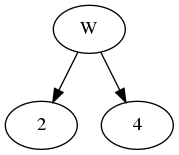
\includegraphics[scale=0.5]{images/Section5applyOnce0}
    \hspace{2cm}
    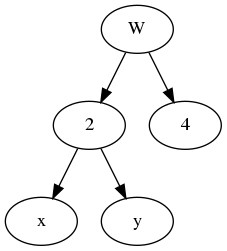
\includegraphics[scale=0.5]{images/Section5applyOnce1}
    \caption{The result of calling applyOnce in Listing \ref{lst:applyOnce} on the Left diagram with a rule }
    \label{fig:applyOnce}
\end{figure}




We now examine applyOnceWithSkip, which builds on applyOnce to deliver more functionality.
This is our key function from Section \ref{design} for solving the problem of replicating rule application in a particular place in an expression.


This function is very similar to the previous one. We add an input parameter 'skip', which is an int representing how many successful rule applications to skip during the expression traversal. If our rule application is successful, but skip is still positive, then we decrement skip and continue the traversal.

\begin{lstlisting}[caption={The same as Listing \ref{lst:applyOnce}, but with an additional skip parameter n which will 'skip' n successful rule applications before returning the result of a successful one}, label={lst:applyOnceWithSkip}]
    def applyOnceWithSkip(t: Tree, skip: Int, r: Strategy[Tree]): (Int, RewriteResult[Tree]) = {

      def recurse(skip: Int): (Int, RewriteResult[Tree]) = {/* Handle the recursive case */}

      r(t) match {
        case Success(newT) =>
          if (skip == 0) {
            (0, Success(newT))
          } else {
            recurse(skip - 1)
          }
        case Failure(_) =>
          recurse(skip)
      }
    }
\end{lstlisting}

Naturally, if you pass a skip value of 0, then this function works exactly the same as applyOnce.
However, this algorithm is inefficient, as the same computations are repeated n times for an initial skip value of n and enough possible successful rule applications. It is not true in general that the number of successful rule applications is known, and so we will need to develop functions later on to figure this out. For the purposes of this function, it is assumed to be known. 


Figure \ref{fig:applyOnceWithSkip} shows the result of applyOnceWithSkip with the same input expression and rewrite rule as Figure \ref{fig:applyOnce}, but with a skip value of 1. Note how during the preorder traversal, we visit the leftmost leaf node first, but as we passed a skip value of 1, we do not stop the traversal here. We continue to the right leaf node, and with our decremented skip value of 0, we return the result of the successful rule application on the right lead node.


\begin{figure} 
    \centering
    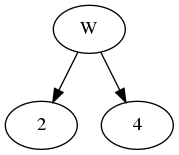
\includegraphics[scale=0.5]{images/Section5applyOnceWithSkip0}
    \hspace{2cm}
    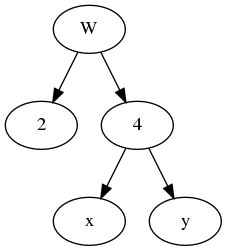
\includegraphics[scale=0.5]{images/Section5applyOnceWithSkip1}
    \caption{An example of calling the function in Listing \ref{lst:applyOnceWithSkip} with skip value of 1 in on the Left expression, with the same rewrite rule as in Figure \ref{fig:applyOnce}}
    \label{fig:applyOnceWithSkip}
\end{figure}





\subsection{applyOnceNTimes and applyOnceNTimesReturnSkip}

We now move to develop functions that can return multiple trees from all possible successful rule applications on an expression. applyOnceNTimes returns a set of trees representing the result of all possible successful rule applications of a single rule on a single expression.

\begin{lstlisting}[caption={???}, label={lst:applyOnceNTimes}]
    def applyOnceNTimes(t: Tree, r: Strategy[Tree], set: Set[Tree]): Set[Tree] = {
      applyOnceWithSkip(t, set.size, r) match {
        case (_,Failure(_)) => set // we are done, couldn't find a rule application that resulted in something new
        case (_,Success(newT)) =>
          t match {
            case EmptyNode => set + newT // we succeeded in rule application, but can't recurse anymore
            case Node(lt, v, rt) =>
              applyOnceNTimes(t, r, set + newT) // keep calling this function until applyOnceWithSkip fails.
            // Each success should add an element to the set,
            // and for an n node tree, at most n elements should be added to the set
          }
      }
    }
\end{lstlisting}


We utilise applyOnceWithSkip from Listing \ref{lst:applyOnceWithSkip} to progressively build up a set of the possible resultant trees. By continually calling applyOnceWithSkip, increasing the skip parameter each time until it fails, we ensure that every node is tried, and all nodes that the rule is successfully applied to have their result added to our set. 
Thus, we now have a function that can tell us where one particular rule can get us to in one step. Remember, we are building to multiple rules across multiple steps.



To solve our earlier problem with applyOnceWithSkip where we don't know in advance how many skips we want, Listing \ref{lst:applyOnceNTimesReturnSkip} presents a version of Listing \ref{lst:applyOnceNTimes} that also returns how many skips were required to get each resultant tree in the set.

\begin{lstlisting}[caption={The same as Listing \ref{lst:applyOnceNTimes}, except that we return how many skips each resultant tree took to achieve}, label={lst:applyOnceNTimesReturnSkip}]
    def applyOnceNTimesReturnSkip(t: Tree, r: Strategy[Tree], set: Set[(Tree, Int)]): Set[(Tree, Int)] = {
      applyOnceWithSkip(t, set.size, r) match {
        case (_,Failure(_)) => set //
        case (_,Success(newT)) =>
          t match {
            case EmptyNode => set + Tuple2(newT, set.size)
            case Node(lt, v, rt) =>
              applyOnceNTimesReturnSkip(t, r, set + Tuple2(newT, set.size))
          }
      }
    }
\end{lstlisting}

Now we have a complete set of functions that allow us to find out what possible trees we can get as a result of applying a single rewrite rule one time, and we have developed a method for recreating all of these transformations. 
We now begin answering our question of whether we can turn one expression into another, building progressively improving transformers.



\section{Expression Transformers}

At this point, we have all the components necessary to begin answering the question of "Can we get from one expression to another using rules X, Y, and Z?"

\subsection{naiveExpressionTransformer and naiveExpressionTransformerReturnOrder}

This expression transformer takes a start and goal expression, a set of rules with which to achieve the transformation, and an integer 'depth' representing the maximum number of rule applications before giving up.

 
Listing \ref{lst:naiveExpressionTransformer} lays out the implementation for our first expression transformer. Because we are ignoring efficiency and performance, the "naïvety" is that there is an exponential time complexity which increases with the number of possible successful rule applications. This is because after collating the set of all resultant trees by calling applyOnceNTimes for each rule, we recurse on all of these different trees, unlike with our binary tree traversals, which are still exponential, but only order $2^n$, where n is the depth of the tree.


\begin{lstlisting}[caption={The first and simplest expression transformer}, label={lst:naiveExpressionTransformer}]
def naiveExpressionTransformer(begin: Tree, goal: Tree, rules: Set[Strategy[Tree]], depth: Int): Boolean = {
    if (depth == 0) return false
    
    var candidates : Set[Tree] = Set()
    for (rule <- rules) {
        val rulecans = applyOnceNTimes(begin, rule, Set())
        candidates ++= rulecans
    }
    // candidates should now hold all possible expressions we could get from successfully applying one of the rules in the provided set once.
    
    for (can <- candidates) {
        if (can == goal) return true
    }
    for (can <- candidates) if (naiveExpressionTransformer(can, goal, rules, depth - 1)) return true
    return false // if all else fails
}
\end{lstlisting}


This transformer only outputs whether it found a possible transformation, and not how to recreate it. To do that, we must return the rules used, in order, and the number of skips in a preorder traversal before applying each rule.
% Could be good as well to show an example with like 10 figures for each of the resultant trees from two rules and a starting expression. But take care as the function only outputs whether the transformation is possible, not how it was found/done.






Our next transformer will tell us not only if the transformation was possible, but also the rules used to do the transformation, in order of application.

\begin{lstlisting}[caption={The same as Listing \ref{lst:naiveExpressionTransformer}, except that it returns the order in which rules are applied if successful}, label={naiveExpressionTransformerReturnOrder}]
def naiveExpressionTransformerReturnOrder(begin: Tree, goal: Tree, rules: Set[Strategy[Tree]], depth: Int, appOrder: Seq[Strategy[Tree]]): (Boolean, Seq[Strategy[Tree]]) = {
  if (depth == 0) return (false, Seq()) 

  // we track which rule led to which resultant trees, so we can return the order
  var candidates : Set[(Strategy[Tree],Set[Tree])] = Set()
  for (rule <- rules) {
    val rulecans = applyOnceNTimes(begin, rule, Set()) // rulecans has type Set[Tree]
    candidates += Tuple2(rule , rulecans)  // that is to say, the trees in the set on the right got there from the rule on the left
  }


  for ((rule, rulecans) <- candidates) {
    for (can <- rulecans) if (can == goal) return (true, appOrder :+ rule)
  }

  // we couldn't find a succesful rule application in this iteration, go deeper
  for ((rule, rulecans) <- candidates) {
    for (can <- rulecans) {
      naiveExpressionTransformerReturnOrder(can, goal, rules, depth-1, appOrder :+ rule) match {
        case (true, newAppOrder) => return (true, newAppOrder)
        case (false, _) => (false, Seq()) // just keep going, next can
        case _ => ??? // panic
      }
    }
  }

  return (false, Seq())
}
\end{lstlisting}

Things get interesting here as there may be more than one solution. That is, more than one way to achieve the transformation from start to goal expression using certain rules. And some methods may be more desirable than others. 
But, as there is no priority or preference given to any particular rule, this means that we might find a solution that takes much longer than is necessary. 

The good news is that even if the transformation is possible within the prescribed depth, all of our transformers will still find that one way to achieve it. This is due to the fact that we simply try every possible combination of rules against every node in our starting tree, as well as all intermediate trees. We can stop if at any point one of our resultant trees is in fact the goal expression.





\subsection{universalExpressionTransformer}

The difference between our previous two transformers and this one is that it returns a way for the solution found to be recreated using applyOnceWithSkip from Listing \ref{lst:applyOnceWithSkip} iteratively with each returned rule and skip value. Listing \ref{lst:universalExpressionTransformer} presents this final function which completes our interface.

\begin{lstlisting}[caption={Our final traversal function, which returns the exact method of recreating a transformation from on expression to the other}, label={lst:universalExpressionTransformer}]
    
def universalExpressionTransformer(begin: Tree, goal: Tree, rules: Set[Strategy[Tree]], depth: Int, appOrder: Seq[Tuple2[Strategy[Tree], Int]]) : (Boolean, Seq[Tuple2[Strategy[Tree], Int]]) = {
    if (depth == 0) return (false, Seq())

    // we track which rule led to which resultant trees, as well as the number of skips for each tree-rule combination
    var candidates : Set[( Strategy[Tree] , Set[(Tree, Int)] )] = Set()
    for (rule <- rules) {
        val rulecans = applyOnceNTimesReturnSkip(begin, rule, Set()) // rulecans has type Set [ (Tree , int) ]
        candidates += Tuple2(rule , rulecans)
    }
    
    for ((rule, rulecans) <- candidates) {
        for ((can, skips) <- rulecans) {
            if (can == goal) return (true, appOrder :+ (rule, skips))
        }
    }
    
    for ((rule, rulecans) <- candidates) {
        for ((can, skips) <- rulecans) {
            universalExpressionTransformer(can, goal, rules, depth-1, appOrder :+ (rule, skips)) match {
                case (true, newAppOrder) => return (true, newAppOrder)
                case (false, _) => (false, Seq()) // just keep going
                case _ => ???
            }
        }
    }
    
    return (false, Seq())
    }
\end{lstlisting}


Talk about it here again




final thoughts on the interface / function suite as a whole that we have developed.






%==================================================================================================================================
\chapter{Evaluation} \label{evaluation}

In this section, we will take a look at a concrete implementation of the ideas discussed in the previous section, through a case study. We have encoded actual transformation rules that correspond to mathematical properties and our trees that rules are applied to represent mathematical expressions (such as 3 * (4 + 5) => (3 * 4) + (3 * 5))


\section{Case Study: Arithmetic Expressions}

No evaluation of expressions implemented. 
Expressions are structured similarly to Reverse Polish Notation. Our nodes are values, or are operators whose two children are that operations arguments.
The rewrite rules we encoded for these Mathematical properties never change the value of the expression, just how it is written.
Thus at end of section, talk about how this could be used to prove that much more complicated expressions are actually equal. 
With the obvious follow on coming back to section 3 requirements that we could have chosen rewrite rules that work on a program AST and thus proved equivalence between high level Lift programs and their low level optimised counterparts.


\subsection{Associativity as a rewrite rule}

Associativity is the property that both Addition and Multiplication have, where the order you do multiple Additions in does not affect the result. For example, (3 + 4) + 5 is the same as 3 + (4 + 5).

For the sake of modularity we define left and right Associativity (swapping the left argument and right argument respectively) separately, but put together they offer all the same capabilities that we need for the Full Associativity Addition and Multiplication.


To illustrate our implementation, here is how it interacts with the aforementioned (3 + 4) + 5.


\begin{figure}
    \centering
    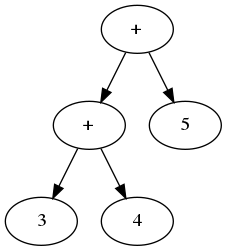
\includegraphics[scale=0.5]{images/Associativity0}
    \hspace{2cm}
    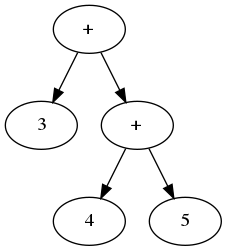
\includegraphics[scale=0.5]{images/Associativity1}
    \caption{Left: The expression representing (3 + 4) + 5; Right: The result of applying our Associativity rule to the left expression}
    \label{fig:Associativity_Example}
\end{figure}




\begin{lstlisting}
// Associativity - Order of Operations irrelevant - Order of two or more of "+" or "*" in same precedence doesn't matter
case class LeftAssociativity() extends Strategy[Tree] {
    def apply(e: Tree): RewriteResult[Tree] = e match {
        case Node(lr, v, c) if v == "+" || v == "*" =>
        lr match {
            case Node(a, v1, b) if v1 == v =>
                Success(Node(a, v, Node(b, v, c))) // (a + b) + c == a + (b + c)
            case _ => Failure(LeftAssociativity())
        }
      case _ => Failure(LeftAssociativity())
    }
}

// Similarly for Right Associativity...
\end{lstlisting}





\subsection{Commutativity}

Commutativity is the simplest of the three properties; It simply means you can swap the arguments in an Addition or Multiplication freely.




\begin{lstlisting}
    case class Commutativity() extends Strategy[Tree] {
        def apply(e: Tree): RewriteResult[Tree] = e match {
          case Node(lr, v, rt) if v == "+" || v == "*" =>
            Success(Node(rt, v, lr)) // sub a + b => b + a
          case _ => Failure(Commutativity())
        }
    }
\end{lstlisting}





\subsection{Distributivity}

Distributivity is a bit more involved than the previous two, since it requires two functions in it's definition. Simply put, if Multiplication distributes over Addition, then any multiplication that has an Addition as one of its operators then the expression can be rewritten into two separate multiplications.

This is best illustrated with another diagram.




\begin{lstlisting}
// Distributivity - Multiplication distributes over Addition i.e.  a * (b + c) == (a * b) + (a * c)
  case class Distributivity() extends Strategy[Tree] {
    def apply(e: Tree): RewriteResult[Tree] = e match {
      case Node(a, v, rt) if v == "*" =>
        rt match {
          case Node(b, v1, c) if v1 == "+" =>
            Success(Node(Node(a, "*", b), "+", Node(a, "*", c))) // a * (b + c) => a*b + a*c
          case Node(b, v1, c) if v1 == "-" =>
            Success(Node(Node(a, "*", b), "-", Node(a, "*", c))) // a * (b - c) => a*b - a*c 
          case _ => Failure(Distributivity())
        }
      case _ => Failure(Distributivity())
    }
  }
\end{lstlisting}



\section{Examples}
\subsection{Simple Example}

We now look at a small example in practice, and evaluate it.


If we create trees which represent the expressions (3 + 4) * 5 and (5 * 3) + (5 * 4) as in Figure ~\ref{fig:CommutDis_Example}, we can see that we can go from the left expression to right expression by first applying the Commutativity rule on the multiplication, and then splitting the multiplication in two using the Distributivity rule.


\begin{figure}
    \centering
    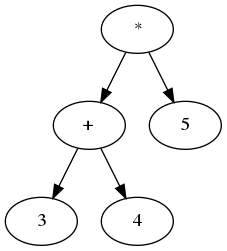
\includegraphics[scale=0.4]{images/CommutDis0}
    \hspace{1cm}
    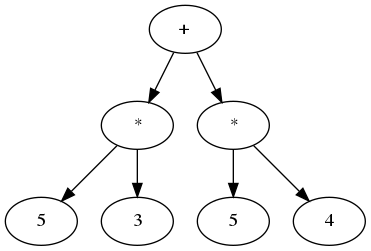
\includegraphics[scale=0.4]{images/CommutDis4}
    \caption{Start and Goal expressions}
    \label{fig:CommutDis_Example}
\end{figure}



We now take a look at what happens when we call our universalExpressionTransformer with these start and goal expressions.
Indeed, we learn that it is possible as it should be, but the method provided to do so is far from the optimal two stage rule application we desire.

Interestingly, the function commutes the Addition arguments first, then commutes them again, resulting in the original starting expression. No progress has been made. Then it finds the solution to commute the Multiplication and apply Distributivity. The solution it presents is double the length of the optimal one, but it does indeed find a solution.


We now evaluate how the function fares on much more complex expressions.

\subsection{Complex Examples}


\subsection{Other stuff}
What problem did my implementation try to address? = Subset of the more general and ambitious "Performance portability and programmability" = possible proof of concept for extension to actual Lift programs that, along with other related work (cite other things here), could show how the low level optimised code the Lift spits out is a valid implementation of whatever high level algorithm the user has written.




%==================================================================================================================================
\chapter{Conclusion}    


\section{Research Outcomes}
Can talk about what found from Dis.
Talk about troubles I had,
What to improve in a future project
What future work could actually be done (furthering this project)

\section{Future Work}
\section{Conclusion}



Summarise the whole project for a lazy reader who didn't read the rest (e.g. a prize-awarding committee).
\section{Guidance}
\begin{itemize}
    \item
        Summarise briefly and fairly.
    \item
        You should be addressing the general problem you introduced in the
        Introduction.        
    \item
        Include summary of concrete results (``the new compiler ran 2x
        faster'')
    \item
        Indicate what future work could be done, but remember: \textbf{you
        won't get credit for things you haven't done}.
\end{itemize}


\
 - What did i do?
 - How did it (maybe) help with Performance Portability and Programmability.
 - Summary of results
 - Future work (already spoken about by this point but reiterate briefly the point of the whole thing)





%==================================================================================================================================
%
% 
%==================================================================================================================================
%  APPENDICES  

\begin{appendices}

\chapter{Appendices}

Only possible thing i can think of would be source code directory structure.

\end{appendices}

%==================================================================================================================================
%   BIBLIOGRAPHY   

% The bibliography style is abbrvnat
% The bibliography always appears last, after the appendices.

\bibliographystyle{abbrvnat}

\bibliography{l4proj}

\end{document}
